% Gemini theme
% https://github.com/anishathalye/gemini
%
% We try to keep this Overleaf template in sync with the canonical source on
% GitHub, but it's recommended that you obtain the template directly from
% GitHub to ensure that you are using the latest version.

\documentclass[final]{beamer}

% ====================
% Packages
% ====================

\usepackage[T1]{fontenc}
\usepackage{lmodern}
\usepackage[size=custom,width=84.1,height=118.9,scale=1.2]{beamerposter}
\usetheme{gemini}
\usecolortheme{edinburgh}
\usepackage{graphicx}
\usepackage{booktabs}
\usepackage{tikz}
\usepackage[numbers]{natbib}
\usetikzlibrary{shapes, arrows, positioning, fit, calc, arrows.meta}
\usetikzlibrary{bayesnet, positioning}
\tikzset{>=latex}

\bibliographystyle{abbrvnat}

% ====================
% Lengths
% ====================

% If you have N columns, choose \sepwidth and \colwidth such that
% (N+1)*\sepwidth + N*\colwidth = \paperwidth
\newlength{\sepwidth}
\newlength{\colwidth}
\newlength{\doublewidth}
\setlength{\sepwidth}{0.0333\paperwidth}
\setlength{\colwidth}{0.45\paperwidth}
\setlength{\doublewidth}{0.933\paperwidth}

\setlength{\abovecaptionskip}{0.5ex}

\newcommand{\separatorcolumn}{\begin{column}{\sepwidth}\end{column}}

\definecolor{phicolor}{HTML}{0074D9}
\definecolor{gammacolor}{HTML}{FF851B}

% Tikz options
\tikzset{%
  var/.style      = {draw, thick, circle, minimum size=0.6cm, inner sep=0},
  block/.style    = {draw, thick, rectangle, rounded corners},
  customline/.style    = {draw opacity=0.4, line width=1}
}
\tikzstyle{arrow} = [draw,line width=0.8pt, black, >=triangle 45]

\definecolor{b}{rgb}{0, 0, 0}
\definecolor{g}{rgb}{0, 0, 0}
\definecolor{r}{rgb}{0, 0, 0}
\definecolor{m}{rgb}{0, 0, 0}

\newcommand{\bx}{\mathbf{x}}
\newcommand{\bv}{\mathbf{v}}
\newcommand{\bm}{\mathbf{m}}
\newcommand{\bb}{\mathbf{b}}
\newcommand{\bc}{\mathbf{c}}
\newcommand{\bd}{\mathbf{d}}
\newcommand{\bs}{\mathbf{s}}

% ====================
% Title
% ====================

\title{Scalable Extreme Deconvolution}

\author{James A. Ritchie, Iain Murray}

\institute[]{School of Informatics, University of Edinburgh}

% ====================
% Body
% ====================

\begin{document}

\addtobeamertemplate{headline}{} 
{
    \begin{tikzpicture}[remember picture,overlay] 
    \node [anchor=north west, inner sep=3cm] at ([xshift=0.cm, yshift=1.cm]current page.north west)     
    {
\includegraphics[height=4.cm]{figures/uoe-informatics-white.png}}; 
    \end{tikzpicture} 
}

\addtobeamertemplate{headline}{} 
{
    \begin{tikzpicture}[remember picture,overlay] 
    \node [anchor=north east, inner sep=3cm] at ([xshift=0.cm, yshift=1.cm]current page.north east)     
    {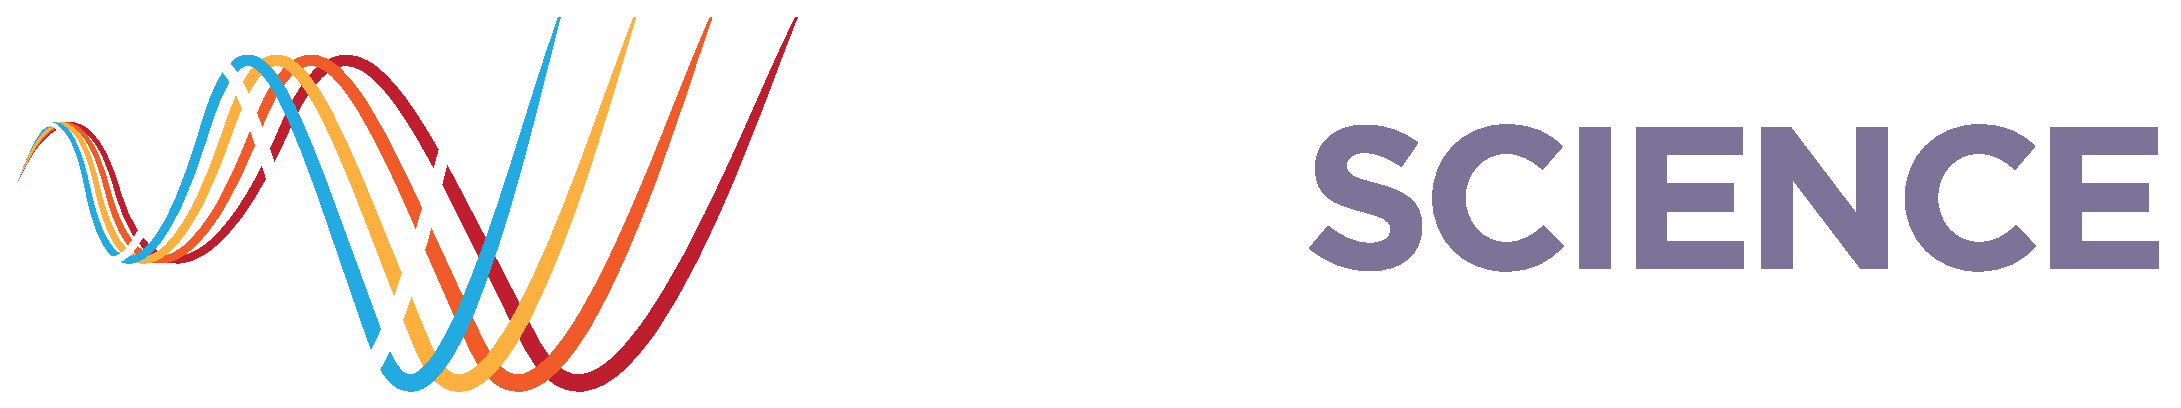
\includegraphics[height=3.cm]{figures/cdt-inverted.eps}}; 
    \end{tikzpicture} 
}

\addtobeamertemplate{headline}{} 
{
    \begin{tikzpicture}[remember picture,overlay] 
    \node [anchor=north east, inner sep=3cm] at ([xshift=0.cm, yshift=-3.cm]current page.north east)     
    {
\includegraphics[height=3.cm]{figures/epsrc_logo.pdf}}; 
    \end{tikzpicture} 
}

\begin{frame}[t]

\begin{columns}[t]

\separatorcolumn
\begin{column}{\doublewidth}
\vspace{-3ex}
\begin{figure}
        \centering
        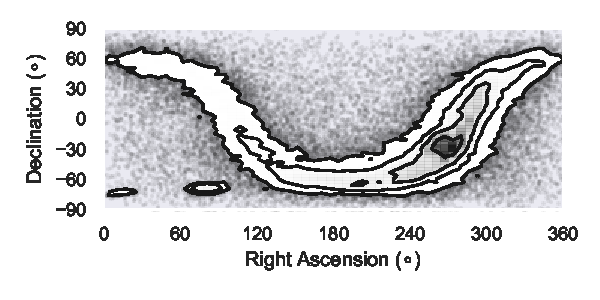
\includegraphics{figures/density.pdf}
        \caption{Marginalised log-density plot of an extreme deconvolution model with $K=256$ components, fitted with our minibatch EM method to a subset of the Gaia astronomical catalogue. The plot shows the estimated density of star positions on the sky, and has correctly recovered the structure of the Milky Way and the Magellanic Clouds.}
\end{figure}
\vspace*{2ex}
\end{column}

\separatorcolumn

\end{columns}

\begin{columns}[t]
\separatorcolumn

\begin{column}{\colwidth}
    
    \begin{alertblock}{Summary}
        \begin{itemize} 
            \item \textbf{Extreme Deconvolution} is a method for fitting \textbf{Gassian Mixture Models} to noisy data, originally intended for use with astronomical datasets.
            \item We propose two \textbf{stochastic minibatch methods} for fitting such models which can run on GPUs. 
            \item Our methods \textbf{converge faster} and take less time to fit with \textbf{larger models} compared to the existing batch method.
        \end{itemize}
    \end{alertblock}
    
    \begin{block}{Extreme Deconvolution}
        We have noisy $d$-dimensional data $\{\bx_i\}_{i=0}^N$,
        \begin{equation}
            \bx_i = \bv_i + \epsilon_i,\quad  \epsilon_i \sim \mathcal{N}(\mathbf{0}, S_i),
        \end{equation}
        where we know the noise covariance $S_i$.
        We want to fit a Gaussian Mixture Model (GMM) with $K$ components to $\bv$,
        \begin{equation}
        p(\bv_i \mid \theta) = \sum_j^K \alpha_j \,\mathcal{N}(\bv_i \mid \bm_j, V_j), \quad \theta = \{\alpha_j, \bm_j, V_j\}_{j=1} ^ K.
        \end{equation}
        As the noise model is Gaussian and the model of the underlying density is a mixture of Gaussians, the probability of $\bx_i$ is also a Gaussian mixture with total log-likelihood
        \begin{equation}
        \mathcal{L}(\theta) = \sum_i^N \log \sum_j^K \alpha_j\,\mathcal{N}(\bx_i \mid \bm_j, T_{ij}), \quad T_{ij} = V_j + S_i.
        \end{equation}
        \citet{bovyExtremeDeconvolutionInferring2011} present a batch method for fitting this model using an Expectation-Maximisation (EM) method, originally intended for astronomical datasets.
        We propose two new methods for fitting this model that scale to larger models for use with larger datasets.
    \end{block}

    \begin{block}{Method 1: Minibatch Expectation-Maximisation}
        \begin{itemize}
        \item Following~\citet{cappeOnlineExpectationMaximization2009}, we develop a minibatch version of the EM procedure.
        \item At each iteration $t$ compute sums of expected sufficient statistics $\phi_{jt}$ per mixture component $j$ over a minibatch.
        \item Stochastic estimates $\hat{\phi}_{jt}$ then updated with a sufficiently small step size $\lambda$,
        \begin{equation}
        \hat{\phi}_{jt} = (1 - \lambda)\hat{\phi}_{j(t-1)} + \lambda \phi_{jt}.
        \end{equation}
        \item Normalise $\hat{\phi}_{jt}$ after each iteration to update the parameters.
        \item If we set $\lambda=1$ and replace each minibatch with the entire dataset, then the update corresponds to the original batch fitting method.
        \end{itemize}
    \end{block}

    \begin{block}{Method 2: Stochastic Gradient Descent}
        \begin{itemize}
            \item We can also optimize the likelihood directly with respect to the parameters $\theta$.
            \item Following \citet{williams1996}, we transform the parameters to remove constraints.
            \begin{itemize}
                \item For the mixture weights $\alpha_j$, we take a softmax of an unconstrained vector $\mathbf{z}$,
                \begin{equation}
                \alpha_j = \frac{e^{z_j}}{\sum_{k=1}^K e^{z_k}}.
                \end{equation}
                \item For the covariances $V_j$, we represent them as a lower triangular Cholesky decomposition $L_j$, where the diagonal elements $qq$ of $L_j$ are constrained positive by taking the exponential of unconstrained elements $\tilde{L}_q$,
                \begin{equation}
                V_j = L_jL_j^T, \quad
                (L_j)_{qq} = \exp({\tilde{L}_q}).
                \end{equation}
            \end{itemize}
            \item With no constraints, we can use any standard minibatch gradient-based optimiser.
        \end{itemize}
    \end{block}
    
\end{column}

\separatorcolumn

\begin{column}{\colwidth}
    \vskip0.5ex
    \begin{block}{Experiments}

        \begin{itemize}
        \item We fitted extreme deconvolution models to a random subset of data from the Gaia DR2 Catalogue~\cite{brownGaiaDataRelease2018}.
        \item Our methods running on GPUs were compared against the reference implementation provided by~\citet{bovyExtremeDeconvolutionInferring2011} running on CPU.
        \item Both of our methods converged faster and took less time to fit, with slightly improved test log-likelihoods.
        \item The SGD method was more numerically stable than the minibatch EM method.
        \item More experiments are needed to demonstrate the utility of our methods for real astronomical problems.
        \end{itemize}

        \begin{figure}
        \centering
        \includegraphics{figures/plots/epochs.pdf}
        \caption{Average training log-likelihood as a function of training epoch for models with $K=256$ components. Epochs rescaled by average training time. Error bars indicate $\pm$ 2 standard deviations.}
        \end{figure}

        \begin{figure}
        \centering
        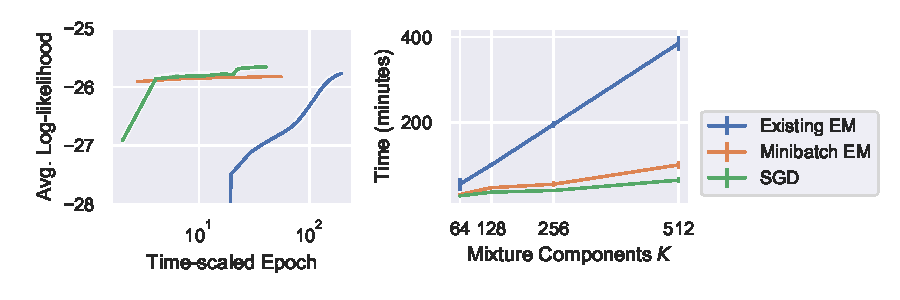
\includegraphics{figures/plots/learning.pdf}
        \caption{Training time as a function of mixture components $K$. Error bars indicate $\pm$ 2 standard deviations.}
        \end{figure}
    \end{block}

    \begin{block}{References}

    \footnotesize{\bibliography{poster}}

    \end{block}
    
\end{column}

\separatorcolumn
\end{columns}
\end{frame}

\end{document}
